\documentclass[10pt,letterpaper]{article}
\usepackage[margin=0.75in]{geometry}
\usepackage[T1]{fontenc}
\usepackage{lmodern,microtype,booktabs,graphicx,amsmath}
\usepackage[font=small,labelfont=bf]{caption}
\usepackage[hidelinks]{hyperref}
\setlength{\parindent}{0pt}
\setlength{\parskip}{4pt}
\setlength{\textfloatsep}{9pt}
\setlength{\intextsep}{7pt}
\newcommand{\topic}[1]{\par\smallskip\textbf{#1}\quad}
\begin{document}
\begin{center}
{\Large\bfseries CSC311 Project Proposal}\par
{\small Group: [GROUP NUMBER] \quad Members: [NAME 1], [NAME 2], [NAME 3]}\par
\end{center}
\vspace{-1em}
\section{Data Exploration}
% Integrates the team's Google Docs Data Exploration draft (read 2026-10-24)
% with the canonical-training notebook results. The source draft is at:
% https://docs.google.com/document/d/1WI5J3QOiBmFf1tvhM9RKkNiCqrfUKuaGP36yjEjsIC8/edit
\topic{Dataset and evaluation boundary.}
The dataset contains 870 responses from 290 respondents, each answering for
Soccer, Baseball, and Basketball. The 12 inputs comprise a numerical ease rating
(Q1), three ordinal agreement questions (Q2--Q4), three multi-select questions
(Q5--Q7), four text associations (Q8--Q11), and a text payment response (Q12).
We exclude respondent ID from model inputs because it identifies the contributor
rather than the sport.

Using seed 311, we split by respondent into approximately 70\% training,
15\% validation, and 15\% test: 606/132/132 responses from 202/44/44 people.
Each split is class-balanced, so class resampling is unnecessary. Grouping keeps
one person's responses together, reducing leakage through writing style or
personal preferences. All exploration below uses training data only; validation
is reserved for model selection and the local test set for final evaluation.
Encoded files preserve the canonical raw split membership. Learned preprocessing
parameters are fitted on training only. The course's hidden staff test set is
separate and may differ from this student sample.

\topic{Numerical and categorical distributions.}
We plotted class-wise histograms for Q2--Q4 on a 1--5 Likert scale, excluding
missing/invalid responses, and compared means and variances (Table~\ref{tab:numeric}).
Soccer and Basketball have similar strategy and injury means; Baseball and
Basketball are closer on individual brilliance. Strategy responses vary most
for Baseball, while injury and individual-brilliance variances are relatively
similar across classes. Q1 has 599 observed values, all within 0--10; fractional
responses and endpoints are retained. Baseball is perceived as harder to start,
but within-class spread indicates overlap. Pairwise Spearman correlations among
Q1--Q4 have absolute values at most 0.338, with no strong pairwise redundancy.

\begin{table}[ht]
\centering\small
\caption{Class-wise training summaries before imputation. Q1 uses 0--10,
Q2--Q4 use 1--5, and Q12 assumes a common monetary unit.}
\label{tab:numeric}
\begin{tabular}{lrrr}
\toprule
Statistic & Soccer & Baseball & Basketball\\
\midrule
Q1 mean (SD) & 6.21 (2.27) & 4.01 (2.06) & 6.06 (2.09)\\
Q2 mean (variance) & 3.97 (0.68) & 3.41 (1.12) & 3.90 (0.56)\\
Q3 mean (variance) & 3.80 (0.84) & 2.90 (1.01) & 3.79 (0.90)\\
Q4 mean (variance) & 2.93 (1.18) & 3.80 (1.04) & 3.62 (1.09)\\
Q12 median & 175 & 50 & 150\\
Q12 mean & 407.91 & 131.19 & 287.01\\
\bottomrule
\end{tabular}
\end{table}

Grouped bars compare option counts/proportions for Q5--Q7. Some options are
similar across classes, whereas winter and hip-hop/rap differ markedly.
A binary indicator's mean is its selection rate. Indoor venue, winter, and hip-hop/rap
show strong marginal class associations, with Cram\'er's $V$ of 0.601, 0.561,
and 0.523. These patterns motivate comparing linear and nonlinear classifiers;
marginal plots alone do not establish nonlinear separability.

\topic{Missingness and inconsistencies.}
We distinguish empty cells, recognized markers such as \texttt{n/a}, and
unparseable payment answers. Table~\ref{tab:missing} uses the encoder's rules;
nonmissing text with no retained tokens is a separate issue. Song missingness
varies by class (1.98\%/6.44\%/7.43\%), suggesting that missingness may carry
signal. Unfamiliarity or lack of an association are possible explanations, not
established causes. We retain response rows; the modelling pipeline adds seven
structured-feature missingness indicators, as described on page~2.

\begin{table}[ht]
\centering\small
\caption{Training missing/unusable percentages; denominator 606 for every question.
Q12 includes 7 blanks and 53 nonblank unparseable answers.}
\label{tab:missing}
\begin{tabular}{lrlrlr}
\toprule
Question & \% & Question & \% & Question & \%\\
\midrule
Q1 Ease & 1.16 & Q5 Venue & 1.16 & Q9 Colour & 1.16\\
Q2 Strategy & 1.32 & Q6 Season & 1.16 & Q10 Song & 5.28\\
Q3 Injury & 1.16 & Q7 Music & 1.16 & Q11 Feeling & 1.16\\
Q4 Individual & 1.32 & Q8 Food & 1.98 & Q12 Payment & 9.90\\
\bottomrule
\end{tabular}
\end{table}

\newpage
\topic{Payment parsing and outliers.}
We applied range and category-validity checks to Q1--Q7, retaining valid scale extremes and rare selections. Explicit IQR-based outlier flagging was limited to Q12; text exploration examined word frequencies and vocabulary coverage rather than systematic text-anomaly detection.

The parser extracts 546 training amounts, converts ranges to midpoints and
\texttt{1k} to 1,000, preserves zeros, and uses stated upper bounds as amounts.
Currency labels are ignored without conversion: only four training responses
contain explicit numerical foreign-currency amounts. This assumes a common unit.
Spelled-out or ambiguous amounts can be unparseable, a parser limitation.

Observed amounts are strongly right-skewed: the overall median is 100, mean
275.72, and maximum 10,000 (Figure~\ref{fig:payment}). We inspect extremes using
the 1.5$\times$IQR rule but retain them: a large amount alone does not establish
an error. The current encoder imputes the 60 unavailable amounts with the
training mean and adds a missingness flag. The mean--median difference motivates
considering robust preprocessing. Modelling now applies $\log(1+x)$ after mean
imputation; median payment imputation remains an untested alternative. The
original exploration exports are unchanged.

\begin{figure}[ht]
\centering
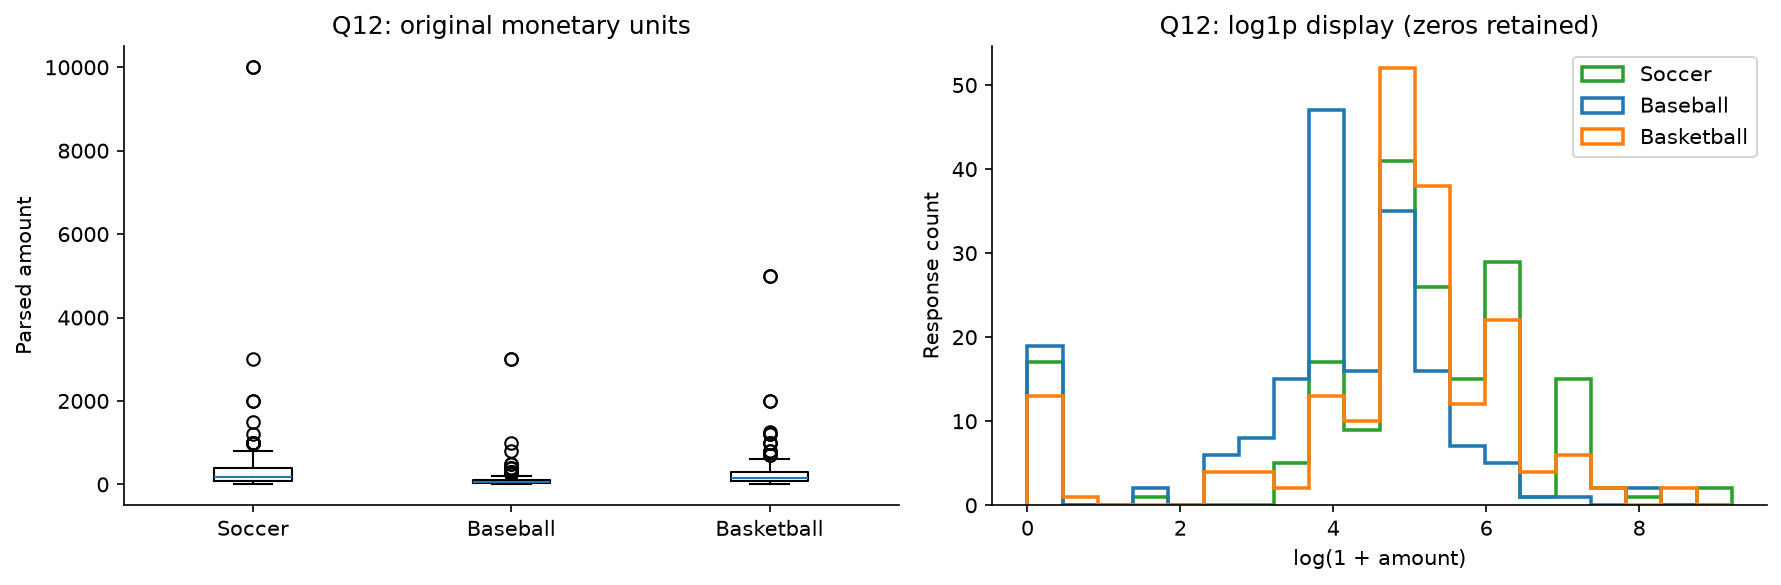
\includegraphics[width=0.84\linewidth]{figures/q12_distribution.png}
\caption{Q12 before imputation: original amounts and a logarithmic view using
common bins across classes. Zeros are retained by $\log(1+x)$.}
\label{fig:payment}
\end{figure}

\topic{Structured-feature representation.}
Q1 is divided by 10; Q2--Q4 map from Strongly Disagree through Strongly Agree to
0, 0.25, 0.5, 0.75, and 1. This preserves order while assuming equal spacing.
Exploratory Likert summaries instead use 1--5. Multi-hot encoding supplies 7 venue,
4 season, and 10 music indicators without imposing an artificial category order.
Multiple indicators can equal one for a response, preserving each selected option.
``Folk or traditional'' and ``classical or jazz'' are each a single music option.
Missing selections remain missing rather than becoming unselected options.
The original Q1--Q7 exports contain 177 missing cells. The modelling pipeline
now imputes numerical/ordinal inputs with training medians and multi-hot inputs
with training modes, adding question-level missingness flags. The original
exports retain raw payment units; model-specific transformations and scaling
are described in Section~\ref{sec:methodology}.

\topic{Text distributions and representation.}
Before vocabulary truncation, normalized food, colour, song, and feeling responses
contained 445, 153, 562, and 599 distinct tokens, respectively, averaging
4.65, 1.95, 4.14, and 4.31 tokens per response containing tokens.
These exploration counts differ from the final TF-IDF vocabularies.
After lowercasing and punctuation normalization, response-level word counts reveal
class-specific signals: ``green'' occurs
in 99 Soccer, 7 Baseball, and no Basketball responses; ``waka'' occurs in 89 Soccer
responses and none of the others. These associations motivate a word-based
representation, though culture and cohort may affect generalization.
Separate TF-IDF encoders retain up to 50 terms each for food, song, and feeling,
and 20 for colour, requiring occurrence in at least two training responses.
Sublinear term frequency reduces repetition effects, inverse document frequency
downweights common terms, and L2 normalization yields weights between 0 and 1.
Vocabulary and IDF are learned only on training; unseen terms are ignored.

Tokens contain at least two A--Z letters; this is an alphabet restriction, not
language detection. Missing text becomes an empty vector plus a missingness flag.
Filtering and vocabulary limits also produce zero vectors for 130 nonmissing song
and 108 nonmissing feeling responses, so zero vectors do not necessarily mean
missing answers. The caps reduce dimensionality but have not been justified by
a model comparison.

\topic{Implications and reproducibility.}
The exploration encoding has 201 predictors; seven structured missingness flags
give 208 in the full-training model fit. Only 202 training respondents and sparse,
overlapping features motivate regularization and fold-local preprocessing.
Plots and audits are in \texttt{analysis/data\_exploration.ipynb}.

\clearpage
\section{Methodology and Development Results}
\label{sec:methodology}
We trained, tuned, and compared multiclass logistic regression, a random forest,
and a small multilayer perceptron (MLP). All experiments used the canonical raw
training split for fitting and grouped cross-validation (CV); external validation
was used only after tuning. The modelling experiments did not access the local
test set, and no final-test performance is claimed. Experiments are reproducible through
\texttt{analysis/model\_comparison.ipynb} and \texttt{analysis/model\_experiments.py}.

\topic{Model families and rationale.}
\textbf{Softmax regression}~\cite{softmax} is a regularized linear baseline that combines evidence
from ordinal responses, multi-hot indicators, and words. It is inexpensive and
interpretable but does not directly learn interactions.
\textbf{Random forest}~\cite{forest} learns thresholds and interactions, such as joint venue and
season associations, while averaging trees to reduce the instability of a single
tree. Deep trees can nevertheless overfit, particularly with sparse word features.
\textbf{MLP}~\cite{mlp} tests learned nonlinear combinations with a single small hidden layer.
With only 202 training respondents, we restricted capacity and tuned regularization
rather than assume a larger network would generalize better. These choices reflect
the observed class associations without claiming that marginal plots establish
nonlinear separability.

\topic{Preprocessing and leakage prevention.}
We excluded ID and label from predictors and retained the existing Q1--Q4 scaling
to $[0,1]$, 21 multi-hot columns, and four separate TF-IDF encoders. Text vocabulary
caps were 50/20/50/50 for food/colour/song/feeling, with minimum document frequency
two, sublinear term frequency, smoothed IDF, L2 normalization, and the existing
alphabet-based tokenizer. Text-missing indicators were retained.

Unknown or invalid structured answers were marked missing. Q1--Q4 were imputed
with training medians and multi-hot columns with training modes, resolving binary
mode ties to zero. Entirely unavailable structured columns had a fixed zero
fallback. Seven question-level missingness indicators were added. Q12 retained
its numeric parser, common-currency assumption, training-mean imputation, and
missingness indicator, followed by $\log(1+x)$. This transformed payment's long
right tail without deleting large amounts. Median payment imputation was not
part of this experiment.

For softmax and MLP, we standardized Q1--Q4 and log-payment using training means
and standard deviations; constant columns used unit scale. Binary indicators and
L2-normalized TF-IDF blocks were unchanged. The forest used the same information
without standardization. The full-training fit had 208 predictors; vocabulary
sizes could vary across folds.

All imputers, vocabularies, IDF weights, and scalers were fitted separately on each
fold's training respondents. Held-out responses were transformed without refitting.
We did not cross-validate the precomputed encoded CSVs. Deterministic preprocessing
was cached within a fold and reused across candidate configurations. Tests verified
that ID/label changes cannot alter inputs, that held-out transformations cannot
change learned parameters, and that missing/unknown structured values yield finite
features.

\topic{Training and hyperparameter search.}
Softmax minimized multinomial cross-entropy with L2 regularization using L-BFGS,
tolerance $10^{-4}$, and a 2,000-iteration limit. MLP used a ReLU hidden layer,
three-class softmax output, cross-entropy, L2 regularization, and L-BFGS with the
same tolerance/iteration limit and at most 50,000 function evaluations. L-BFGS
required neither minibatches nor a manually chosen learning-rate schedule; we did
not use validation-based early stopping. Convergence warnings triggered one retry
with 10,000 iterations and, for MLP, 200,000 function evaluations. Four tuning fits
required retries; all then converged. Selected-model refits had no convergence
warnings.

The forest used 300 bootstrap trees, Gini impurity, no class weights, and one CPU
thread. BLAS computations were also limited to one thread. Depth and minimum leaf
size controlled tree complexity. Out-of-bag scores were not used for selection,
because row-level bootstrapping does not guarantee respondent separation in
out-of-bag evaluation. Software versions included Python 3.12, scikit-learn 1.9.1,
NumPy 2.5.4, and pandas 3.1.0; the run manifest records exact versions and input hashes.

\begin{table}[ht]
\centering\small
\caption{Initial exhaustive searches, using the same five grouped folds for every family.}
\label{tab:search}
\begin{tabular}{lp{0.58\linewidth}r}
\toprule
Family & Hyperparameters & Settings\\
\midrule
Softmax & $C\in\{0.001,0.01,0.1,1,10,100\}$ & 6\\
Forest & Depth $\in\{4,8,12,\text{unlimited}\}$; minimum leaf size
$\in\{1,3,5\}$; \texttt{max\_features}$\in\{\texttt{sqrt},0.5\}$ & 24\\
MLP & Hidden units $\in\{16,32,64\}$;
L2 coefficient $\alpha\in\{0.01,0.1,1,10\}$ & 12\\
\bottomrule
\end{tabular}
\end{table}

\topic{Grouped tuning and boundary checks.}
Within the 606 training responses, five-fold shuffled \texttt{GroupKFold} used
respondent IDs and seed 311. Each person's three responses stayed together, and
folds remained class-balanced. Every family was tuned before comparison. We ranked
configurations by mean CV accuracy, then mean macro-F1, then lower complexity for
exact ties. Smaller $C$ strengthens softmax regularization; larger $\alpha$
strengthens MLP regularization.

The initial grid required 210 fold fits. We checked selected search edges before
opening external validation. Softmax's selected $C=1$ was interior. The forest
selected unlimited depth, minimum leaf size 1, and \texttt{sqrt}; the first two are
natural boundaries. MLP selected 16 units and $\alpha=10$, both initial edges, so
we additionally tested 8 units at $\alpha=10$ and $\alpha=100$ at 16 units.
Their CV accuracies were 89.93\% and 84.82\%, below the selected 90.10\%.
Thus, 44 configurations and 220 fold fits were evaluated. This finite search
supports the selected settings but does not prove global optimality.

Tuning curves showed softmax training accuracy increasing as regularization
weakened, while CV accuracy fell beyond $C=1$, consistent with overfitting.
The best MLP was small and strongly regularized. Selected forest and MLP settings
were repeated on the same folds with seeds 312 and 313, adding 20 fits.
Forest mean CV accuracy ranged from 90.78\% to 91.43\%; MLP ranged from 89.77\%
to 90.10\%. We did not choose a favorable seed: all external-validation refits
used the prespecified seed 311. Fold SDs describe variation, not confidence intervals.

\topic{Metrics and comparison protocol.}
Accuracy was primary, matching the classification task. Macro-F1 gave equal
weight to the three sports, and per-class precision/recall and confusion matrices
were used for error analysis. Undefined precision/F1 denominators were assigned
zero. For class $c$, $F1_c=2\mathrm{TP}_c/(2\mathrm{TP}_c+\mathrm{FP}_c+\mathrm{FN}_c)$;
macro-F1 is the mean of these three values. A constant Soccer classifier achieved
33.33\% validation accuracy and 0.1667 macro-F1.

After tuning, each selected configuration and its preprocessing were refitted on
all 606 training responses and evaluated on the 132 responses from 44 separate
validation respondents. Selection used validation accuracy, then macro-F1, then
a prespecified simpler-family preference for an exact tie. No test data informed
this process. Table~\ref{tab:results} separates training scores, tuning-CV scores,
and model-selection validation scores.

\begin{table}[ht]
\centering\small
\caption{Completed comparison. Accuracy columns are percentages; CV shows mean
$\pm$ sample SD across five folds. Training scores use the full-training refit.}
\label{tab:results}
\begin{tabular}{lrrrrr}
\toprule
Model & Train acc. & CV acc. & CV macro-F1 & Val. acc. & Val. macro-F1\\
\midrule
Softmax & 97.03 & $90.43\pm1.60$ & 0.9039 & 90.91 & 0.9089\\
Forest & 99.34 & $91.27\pm2.14$ & 0.9125 & \textbf{93.18} & \textbf{0.9317}\\
MLP & 96.20 & $90.10\pm2.78$ & 0.9007 & 90.91 & 0.9085\\
\bottomrule
\end{tabular}
\end{table}

\topic{Selected settings and error analysis.}
Softmax selected $C=1$; forest selected 300 trees, unlimited depth, minimum leaf
size 1, and \texttt{sqrt} candidate features; MLP selected 16 hidden units and
$\alpha=10$. The forest was selected for continued development, correctly
classifying 123/132 validation responses, compared with 120/132 for both other
families. Its advantage is only three responses, and CV variability is larger
than the differences between family means; we do not claim decisive superiority.
All models had higher training than held-out accuracy, particularly the forest.

The forest's validation confusion matrix (rows actual, columns predicted; order
Soccer/Baseball/Basketball) was
$\left(\begin{smallmatrix}39&2&3\\1&41&2\\0&1&43\end{smallmatrix}\right)$.
Soccer had the lowest recall, 39/44 (88.64\%), compared with 41/44 (93.18\%)
for Baseball and 43/44 (97.73\%) for Basketball. Soccer predicted as Basketball
was the largest off-diagonal count (three). Complete class metrics, tuning curves,
seed checks, and all three confusion matrices are saved in the modelling notebook.

\topic{Limitations, reproducibility, and next steps.}
Training-set exploration informed feature engineering before CV, and validation
selected among three families; neither score is an unbiased final-test estimate.
The 132 validation responses represent 44 people. Student cultural associations
may generalize poorly to staff responses. No local test predictions have been evaluated.
After choices are frozen, refitting on training plus validation adds respondents
but spends validation's independent role; test evaluation should then occur once.

Fold assignments, hashes, versions, parameters, diagnostics, predictions, and
models are saved in \path{analysis/out/models/}. Reloaded artifacts reproduced
validation predictions. PCA and clustering were not used. Final submission remains
future work: export forest nodes and preprocessing using the standard library, NumPy, and pandas for
inference, verify prediction equivalence, keep all files within 10\,MB, and check
approximately 60 predictions within one minute without networking. Development
scikit-learn artifacts are not submission-ready.

\topic{AI assistance.}
OpenAI Codex assisted with exploration and modelling code, analysis summaries,
and LaTeX drafting and revision.

\begingroup
\small
\begin{thebibliography}{3}
\setlength{\itemsep}{0pt}
\bibitem{softmax} scikit-learn developers.
\href{https://scikit-learn.org/stable/modules/generated/sklearn.linear_model.LogisticRegression.html}{\textit{LogisticRegression}: API documentation}.
\bibitem{forest} scikit-learn developers.
\href{https://scikit-learn.org/stable/modules/generated/sklearn.ensemble.RandomForestClassifier.html}{\textit{RandomForestClassifier}: API documentation}.
\bibitem{mlp} scikit-learn developers.
\href{https://scikit-learn.org/stable/modules/generated/sklearn.neural_network.MLPClassifier.html}{\textit{MLPClassifier}: API documentation}.
\end{thebibliography}
\endgroup
\end{document}
